\documentclass[12pt]{article}
\usepackage{amsmath, graphicx, caption,array}
\usepackage{amsthm}
\usepackage{amsfonts, xcolor, physics, listings,verbatim}
\usepackage{amssymb,empheq}
\usepackage{mathrsfs}
\usepackage[T1]{fontenc} % for \symbol{92} 
\usepackage{comment, subfig, hyperref, url}
\usepackage{textcomp}

% Command "alignedbox{}{}" for a box within an align environment
% Source: http://www.latex-community.org/forum/viewtopic.php?f=46&t=8144
\newlength\dlf  % Define a new measure, dlf
\newcommand\alignedbox[2]{
% Argument #1 = before & if there were no box (lhs)
% Argument #2 = after & if there were no box (rhs)
&  % Alignment sign of the line
{
\settowidth\dlf{$\displaystyle #1$}  
    % The width of \dlf is the width of the lhs, with a displaystyle font
\addtolength\dlf{\fboxsep+\fboxrule}  
    % Add to it the distance to the box, and the width of the line of the box
\hspace{-\dlf}  
    % Move everything dlf units to the left, so that & #1 #2 is aligned under #1 & #2
\boxed{#1 #2}
    % Put a box around lhs and rhs
}
}

\addtolength{\oddsidemargin}{-1in}
\addtolength{\evensidemargin}{-1in}
\addtolength{\textwidth}{1.75in}
\addtolength{\topmargin}{-1in}
\addtolength{\textheight}{1.75in}
\newcommand{\contra}{$\rightarrow\leftarrow$}
\newcommand{\tb}{  \textbackslash  }
\newcommand{\bj}{\ \Longleftrightarrow \ }

%bailey meche
\begin{document}
%bailey meche
	\begin{center}
		ECMA 33230: Macroeconomic Crises - Spring 2025\\
        Problem Set 1: The Credit Crunch \\
		Due Date: April 14, 2025 \\
        Bailey Meche
	\end{center}


%\section*{Problems}

\begin{enumerate}
    \item[2.] (6 points)  Consider the 2-period credit crunch model discussed in class. Describe what empirical
aspects of the financial crisis the model can capture.
\subsubsection*{Solution.}

The credit crunch model discussed in class captures the following empirical phenomena: collapsed bank collateral, decreased intermediation, and increased interest rate spreads (here, borrowing vs lending rates).

The model can also capture capture less investment by firms (via lower borrowing), unconventional monetary policy, and reductions in deposits via the incentive constraint. 

    \item[3.] (9 points) Consider the 2-period credit crunch model discussed in class. Indicate for each statement below if it’s true or false and give a short explanation. No credit without correct explanation.
    \begin{enumerate}
        \item (3 points) The first best allocation delivers a higher consumption level in the first period, a
        lower consumption level in the second period but overall a higher utility than an inefficient
        equilibrium.
        \subsubsection*{Solution.}

        This depends on where the supply curve lies. If the supply is such that $R^d=R^s$, then first-best pricing consumption is equal to the decentralized consumption for both periods. This indicates that the decentralized allocation is efficient, so utility is equal to first-best pricing.

        If $R^d<R^s$, however, the decentralized problem is inefficient since $c_1>c_1^*$ and $c_2<c_2^*$ where first best allocation consumption is $c^*$. The first best utility $u^*$ is always higher than the inefficient outcome $u$ and will always generate weakly greater utility than the decentralized problem.
        Hence, the statement is false. 

        %Hence, in any case, the statement that first best allocation delivers a higher consumption level in the first period and lower consumption level in the second period is true, but the first best allocation delivers a \emph{higher} consumption level in the second period but overall a higher utility than an inefficient        equilibrium.
        
        % Computing utility for the first best allocation $u^*$ 
        % \begin{align}
        %     u^*(y,N,\beta,R^s)&= \max_{c_1,c_2,s} \ln(c_1^*) + \beta \ln(c_2^*) \notag 
        %     \\ &= \ln\left(\frac{y+N}{1+\beta}\right) + \beta \ln\left(\frac{R^s \beta (y+N)}{1+\beta}\right)\label{1}
        % \end{align}
        %  Computing utility for the decentralized problem $u$
        %  \begin{align}
        %      u(y,N,\beta,R^s,R^d)&= \max_{c_1,c_2,s} \ln(c_1^*) + \beta \ln(c_2^*) \notag 
        %      \\ &= \ln\left( \frac{R^s(y+N)}{\beta R^d + R^s} \right) + \beta \ln\left( R^s \left( y+N - \frac{R^s}{\beta R^d + R^s} \right)\right) \label{2}
        %  \end{align}
        %  Comparing \eqref{1} and \eqref{2}
        %  \begin{align}
        %       %\ln\left(\frac{y+N}{1+\beta}\right) + \beta \ln\left(\frac{R^s \beta (y+N)}{1+\beta}\right) &=^? \ln\left( \frac{R^s(y+N)}{\beta R^d + R^s} \right) + \beta \ln\left( R^s \left( y+N - \frac{R^s}{\beta R^d + R^s} \right)\right)
        %       %\\ \frac{(y+N)^{1+\beta} (R^s\beta)^\beta}{(1+\beta)^{1+\beta}} &=^? \frac{R^s(y+N)}{\beta R^d + R^s}\left( R^s \left( y+N - \frac{R^s}{\beta R^d + R^s} \right)\right)^\beta 
        %       u^* - u =  \eqref{1} - \eqref{2} &=  \ln\left(\frac{\beta R^d + R^s}{R^s(1+\beta)}  \right) + \beta \notag \ln\left(\frac{\beta (y+N)}{(1+\beta) \left( y+N - \frac{R^s}{\beta R^d + R^s} \right)} \right)
        %        \\ &= \ln\left(\frac{\beta R^d + R^s}{R^s(1+\beta)}  \right) + \beta \ln\left(\frac{\beta (N + y) (\beta R^d + R^s)}{(\beta + 1) (\beta N R^d + \beta y R^d + N R^s + y R^s - R^s)}\right)\label{3}
        %  \end{align}
        %  Here, by monotonicity, we have \eqref{3} is strictly decreasing in $y+N$. Using this, 
        %  \[ \begin{cases}
        %      u^* \geq u & \text{if } \frac{R^d}{R^s} \geq  \frac{ (1 + \beta)^\beta + \beta (1 + \beta)^\beta-\beta^\beta}{\beta^{1 + \beta}}
        %      \\ u^* < u & \text{if }  \frac{R^d}{R^s} < \frac{ (1 + \beta)^\beta + \beta (1 + \beta)^\beta-\beta^\beta}{\beta^{1 + \beta}}
        %  \end{cases}\]
        %  with a rough solution around $ \frac{ (1 + \beta)^\beta + \beta (1 + \beta)^\beta-\beta^\beta}{\beta^{1 + \beta}}=3$, indicating that $u^* \geq u$ when $R^d \geq 3 R^s.$         
        %  This threshold function is decreasing in $\beta$ with a minimum value of 3 ($\beta=1$). Hence, for values $0< \beta < 1$, we get $u^* < u$.

        %  Therefore, the statement is true for $R^d<R^s$.
        %  %the likelihood of the planners utility $u^*$ rises when $R^s$ is low.
        
    
     \item (3 points) Bankers have the same optimization problem with or without publicly funded
        equity injections into banks.
        \subsubsection*{Solution.}

        True. For equity injection intervention, bankers have the same profits, incentive constraints, and deposit demand as before (derivation shown in lecture). 
    
     
     \item (3 points) Deposit demand is lower with publicly funded bank deposits.
     \subsubsection*{Solution.}

    %\textcolor{red}{NOT DISCUSSED YET }
    For this government intervention, the banker's problem is given by 
    \begin{align}
            \max_{s,d}\pi =&\max_{d}  R^s(N+d) - R^dd+ (R^s-R^d)T   \label{3cb}
            \\ & s.t. &\begin{cases}
                s \leq N + d + T & (BC)
                \\ \pi \geq \lambda R^s(N+d) + \lambda (R^s - R^d)T & (IC)
            \end{cases}\notag 
    \end{align}
    % and the household's problem with utility as in the lecture 
    % \begin{align}
    %         &\max_{c_1, c_2}  \ln(c_1) + \beta \ln(c_2)
    %         && s.t. &\begin{cases}
    %             c_1 + d + T =y & (t=1)
    %             \\ c_2 = R^d(d+T) + \pi  & (t=2)
    %         \end{cases} \label{3ch}
    %         \\ &&& \iff & c_2 = R^dy + \pi - R^d c_1 \notag  %c_1 = \frac{R^dy + \pi -c_2}{R^d} \notag 
    % \end{align}
    Solving \eqref{3cb}:
    \begin{align*}
        \pi &\geq \lambda R^ss 
        \\ R^s(N+d) - R^dd+ (R^s-R^d)T   &\geq \lambda R^s(N+d+T)
        \\ R^s(N+d+T) - R^sT- R^dd+ (R^s-R^d)T  &\geq \lambda R^s(N+d+T)
        \\  - R^sT- R^dd+ R^sT - R^dT &\geq (\lambda-1) R^s(N+d+T)
        \\ \lambda &\leq 1- \frac{R^d(d+T)}{ R^s(N+d+T)} 
        \\ d &\leq \frac{\left(1-\lambda\right)R^{s}\left(N+T\right)-R^{d}T}{R^{d}-\left(1\ -\lambda\right)R^{s}}
         % \\ R^{d}T-d\left(R^{d}+\left((\lambda-1)\left(N+1\right)+\left(\lambda+1\right)T\right)R^{s}\right) &\geq 0 & \text{(demand)}
         % \\ d= \begin{cases}
         %     %0 & R^d > R^s
         %      \frac{(1-\lambda)}{\lambda}N-T & R^d = R^s 
         %     \\ \frac{R^{d}T}{R^{d}+\left((\lambda-1)\left(N+1\right)+\left(\lambda+1\right)T\right)R^{s}} & (1-\lambda)R^s < R^d < R^s
         % \end{cases} && \text{(demand)}         
    \end{align*}
    From this, we see that the banker's problem has changed. Comparing this with the original demand function,
    \[ R^d = \begin{cases}
        R^s & d=\left( 0,\frac{(1-\lambda)}{\lambda}N\right), \ T=0
        \\ (1-\lambda) R^s \frac{N+d+T  }{d+T} & d \geq \frac{(1-\lambda)}{\lambda}N, \ T \geq 0
    \end{cases}
    \]
    % \[d' = \begin{cases}
    %      \frac{(1-\lambda)}{\lambda}N & R^d = R^s 
    %          \\ \frac{\left(1-\lambda\right)R^{s}N}{R^{d}-\left(1-\lambda\right)R^{s}} & (1-\lambda)R^s < R^d < R^s
    % \end{cases}\]
    % we have  in region $R^d = R^s $ that clearly $d'>d$ as $T>0$. In fact, there is a linear decrease in demand as deposits increase.  In region $R^d < R^s $, suppose it is true that $d'>d$. Let $K= (\lambda-1)\left(N+1\right)+\left(\lambda+1\right)T$
    % \begin{align*}
    %     \frac{R^{d}T}{R^{d}+\left((\lambda-1)\left(N+1\right)+\left(\lambda+1\right)T\right)R^{s}} <  \frac{\left(1-\lambda\right)R^{s}N}{R^{d}-\left(1-\lambda\right)R^{s}} 
    %     \\ T (R^d)^2 - T(1-\lambda)R^d R^s-(1-\lambda)R^s N R^d - (1-\lambda)(R^s)^2 NK &<  0
    %     \\ (1-\lambda)(T+N)R^s R^d + (1-\lambda)(R^s)^2 NK &<T(R^d)^2
    %      \\ T\lambda  + (1-\lambda)N^2 &< N (\lambda+1)T
    %       \\ T &> \frac{(1-\lambda)N^2}{N(1+\lambda)-\lambda}
    % \end{align*}
    % Hence, our supposition that $d'>d$ is equivalent to the statement $T > \frac{(1-\lambda)N^2}{N(1+\lambda)-\lambda}$ which is true when both $T$ and $N$ are greater than 0.5 for all $0<\lambda<1$. Therefore, the statement is true - deposit demand is lower with publicly funded bank deposits.
    % Solving \eqref{3ch}: 
    % \begin{align*}
    %     c_1 &= \frac{y + \frac{\pi}{R^d}}{1+\beta }=  \frac{y+\frac{R^s(N+d) - R^dd - (R^s-R^d)T }{R^{d}}}{1+\beta} = \frac{y+\frac{\left(R^{s}-R^{d}\right)(N+d-T)+R^{d}N}{R^{d}}}{1+\beta}
    %     \\ d&= y - c_1 = \frac{\beta y-\frac{\left(R^{s}-R^{d}\right)(N+d -T)+R^{d}N}{R^{d}}}{1+\beta} & \text{(supply)}
    %     \\ c_2 &= R^dy + \pi - R^d c_1 = R^dy + \pi - R^d \cdot  \frac{y + \frac{\pi}{R^d}}{1+\beta }
    %      = \frac{\beta\left(R^{d}y+\pi\right)}{1+\beta}
    %       \\ &= \frac{\beta}{1+\beta}\left(R^{d}(y+N)+\left(R^{s}-R^{d}\right)(N+d-T)\right)
    % \end{align*}
    % The household's problem has also chanaged. 
    
    
     
    \end{enumerate}
    \item[4.] (23 points) Assume $y = 4$, $\lambda = 0.4$, $R^s = 1.04$, $\beta = 0.98$, $N = 0.5$ are known and households have the same log preferences as in the lecture.
    
    \begin{enumerate}
        \item (3 points) State the policy functions for deposit supply and deposit demand (as functions of known variables and $R^d$).        
        \subsubsection*{Solution.}
        
        Deposit supply $d^s$ and deposit demand $d^d$ are given analytically by:
        \begin{align*}
            d^s &= y - \frac{R^s(N+y)}{\beta R^d + R^s}
            \\ d^d &= \begin{cases}
                \frac{1-\lambda}{\lambda}N &R^d = R^s
                \\ \frac{(1-\lambda)R^sN}{R^d - (1-\lambda)R^s} & (1-\lambda)R^s < R^d < R^s
            \end{cases}.
        \end{align*}
        Plugging in assumed values: 
        \begin{align*}
            d^s &= 4 - \frac{1.04(0.5+4)}{0.98 R^d + 1.04} &= \frac{2 (98 R^d - 13)}{49 R^d + 52}
            \\ d^d &= \begin{cases}
                \frac{1-0.4}{0.4}\cdot0.5 & =\frac{3 }{4}
                \\ \frac{(1-0.4)(1.04)(0.5)}{R^d - (1-0.4)(1.04)} & =\frac{\frac{39}{125}}{R^d - \frac{78}{125}} = \frac{39}{125R^{d}-78} %& d\geq \frac{3}{4}
            \end{cases}%&= \frac{39}{125 R^d - 78}
        \end{align*}
        
        \item[(b)] {(5 points)} Plot the deposit supply and demand as a function of the deposit return $R_d$ when $N = 0.5$. Use Julia to make this plot, plot $R_d$ on the y-axis for a range from 0 to 2, choose a reasonable scale for deposits on the x-axis.
        \subsubsection*{Solution.}

        See Figure \eqref{fig:4b}.

        \begin{figure}%[H]
            \centering
                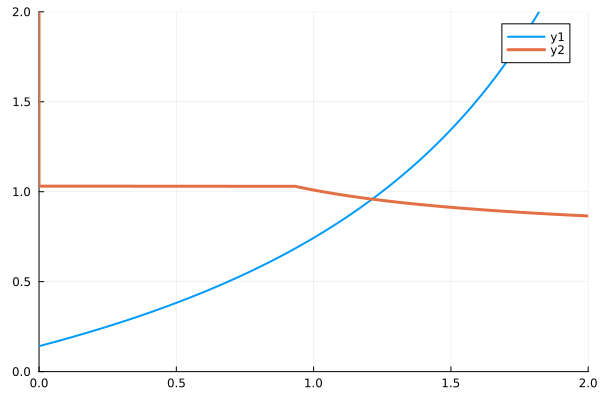
\includegraphics[width=0.7\textwidth]{4b.png}
                \caption{ }
                \label{fig:4b}
        \end{figure}
        
        \item[(c)] {(5 points)} Describe both curves and interpret what happens in each region. \textit{Hint:} When discussing demand, check for $R_d > R_s$, $R_d = R_s$, $(1 - \lambda)R_s < R_d < R_s$, $R_d < (1 - \lambda)R_s$.
        \subsubsection*{Solution.}

        In $R_d > R_s$, with every additional dollar of deposits, banker loses money, so $d=0$. In $R_d = R_s$, banks make zero profits on deposits and incentive constraint is slack (this is the flat region of the orange line). In $(1 - \lambda)R_s < R_d < R_s$, $R_d < (1 - \lambda)R_s$, the bank makes profits on deposits, and incentive constraint binds where $d=\frac{\frac{39}{125}}{R^d - \frac{78}{125}} = \frac{39}{125R^{d}-78}.$
        For the asymptote of $R^d$, we have a lower bound of $R^d = (1-\lambda)R^s.$

        For a discussion of supply from households, households make deposits at an increasing rate with $R^d$. Deposits $d$ are only made at the intersection point with demand.
        
        \item[(d)] {(4 points)} Find the equilibrium by eyeballing the graph. What is the equilibrium deposit rate and deposit quantity? What is the spread? How much profits do banks make?
        \subsubsection*{Solution.}

        See my code that solves for the intersection at ($d = 1.2132$, $R_d = 0.9587$), shown in Figure \eqref{fig:4d}. Here, the spread is 0.071285 where the banks make $0.071285(N+d).$

        \begin{figure}%[H]
            \centering
                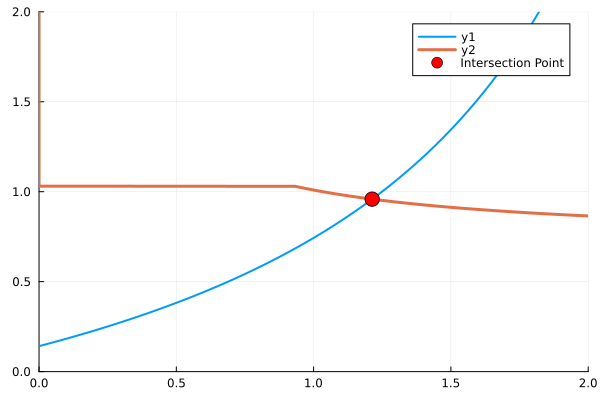
\includegraphics[width=0.7\textwidth]{4d.png}
                \caption{ }
                \label{fig:4d}
        \end{figure}
        
        \item[(e)] {(6 points)} Plot (in the same graph from part (b)) and describe what happens to deposit demand and supply if bankers' net worth has risen to $N = 1.2$ at the beginning of period 1. Provide intuition. What is the value of the spread now?
        \subsubsection*{Solution.}

        See Figure \eqref{fig:4e} for the new demand and supply functions overlayed on Figure \eqref{fig:4b}. The intersection for the functions at $N=1.2$ is at ($d = 0.8687$, $R_d = 1.03$). Now, the incentive constraint is slack since we are in the region where $R^d = R^s$, spread is 0. Demand has moved rightward since $N$ has increased, moving $\frac{\lambda-1}{\lambda}N$. The supply function has shifted rightward by $R^s(N^\text{new}-N^\text{old})$.  The intuition for the shift is by increasing N we increase the payment from the bank the household gets in time 2. Thus they have less incentive to save in time 1. Likewise for demand, the increase in N alters the size of the region where the IC is slack.

        
        \begin{figure}%[H]
            \centering
                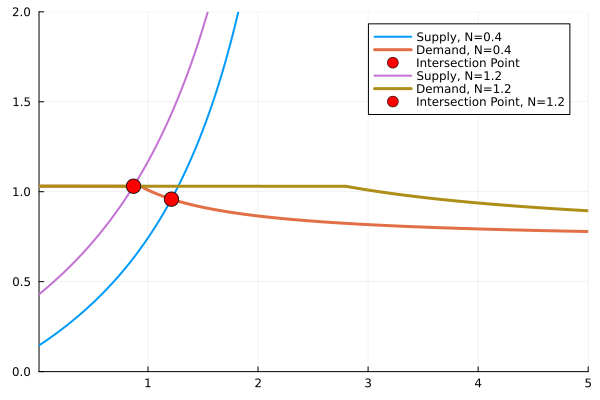
\includegraphics[width=0.7\textwidth]{4e.png}
                \caption{Part (e) }
                \label{fig:4e}
        \end{figure}
        
    \end{enumerate}

 \item[5.] (15 points) Households comprise workers and bankers. Workers earn $y = 1$ in period 1, bankers make profits $\pi$ in period 2 and both types perfectly insure each other’s consumption. Households have preferences over consumption $c_t$:
    \[
    u(c_1, c_2) = \frac{(c_1)^{1-\sigma}}{1 - \sigma} + \beta \frac{(c_2)^{1-\sigma}}{1 - \sigma},
    \]
    where $\beta = \frac{3}{4}$, $\sigma = 2$ and they can earn the deposit return $R_d$ in period 2 on deposits $d$ made in period 1. Bankers’ profits comprise the return $R_s = \frac{4}{3}$ they earn on both their net worth $N = \frac{2}{5}$ and deposits $d$, less the deposit return they have to pay for the latter.
    
    \begin{enumerate}
        \item[(a)] {(3 points)} Set up the intertemporal budget constraint of households. Write down the household’s optimization problem in terms of $y, \beta, \pi, R_d$ and $d$.
        \subsubsection*{Solution.}

        \textbf{Household problem.} Households with perfect household insurance solve the following: 
        \begin{align*}
            &\max_{c_1,c_2,d} u(c_1,c_2) 
            && s.t. &\begin{cases}
                c_1 + d = y & t=1 \\ c_2 = R^d d + \pi & t=2 
            \end{cases}
            \\ &\max _{c_1,c_2,d} \frac{(c_1)^{1-\sigma}}{1 - \sigma} + \beta \frac{(c_2)^{1-\sigma}}{1 - \sigma} && s.t & c_2 = R^d y + \pi - R^d c_1
        \end{align*}
        Taking FOC with respect to  $c_1$: 
        \begin{align*}
            c_1^{-\sigma} + \beta \frac{\partial }{\partial c_1 }\frac{(c_2)^{1-\sigma}}{1 - \sigma}  &= 0
            \\  c_1^{-\sigma} + \beta \frac{\partial }{\partial c_1 }\frac{( R^d y + \pi - R^d c_1)^{1-\sigma}}{1 - \sigma}  &= 0
            \\ c_1^{-\sigma} + \beta (- R^d) ( R^d y + \pi - R^d c_1)^{-\sigma}&= 0
            \\ c_1 &&= \frac{R^{d}y+\pi}{\left(\beta R^{d}\right)^{\frac{1}{\sigma}}+R^{d}}
            \\ d &= y - c_1  &= y - \frac{R^{d}y+\pi}{\left(\beta R^{d}\right)^{\frac{1}{\sigma}}+R^{d}}
            \\ c_2 &= R^d d + \pi &= R^d \left(  y - \frac{R^{d}y+\pi}{\left(\beta R^{d}\right)^{\frac{1}{\sigma}}+R^{d}}\right)  + \pi
        \end{align*}

        This remains incomplete since we haven't said what $\pi$ is. 
        %%% COMPLETE 

        
        \item[(b)] {(5 points)} Find the policy function for deposit supply $d$. Assume the deposit market is in an inefficient equilibrium with $R_d = \frac{16}{27}$. What is the equilibrium deposit level $d_{eq}$?
        \subsubsection*{Solution.}

        Finding supply curve $d$ from optimality condition of households: 
        \begin{align*}
             d  &= y - \frac{R^{d}y+(R^s(N+d) - R^d d )}{\left(\beta R^{d}\right)^{\frac{1}{\sigma}}+R^{d}}% =\frac{y - N R^s (\beta R^d)^\sigma}{R^s (\beta R^d)^\sigma + 1} 
             \\ &= y - \frac{R^{d}y+R^sN +(R^s- R^d) d}{\left(\beta R^{d}\right)^{\frac{1}{\sigma}}+R^{d}}
              \\ d \left(1 + \frac{R^s- R^d}{\left(\beta R^{d}\right)^{\frac{1}{\sigma}}+R^{d}} \right)&= y - \frac{R^{d}y+R^sN}{\left(\beta R^{d}\right)^{\frac{1}{\sigma}}+R^{d}}
               \\  d &= \frac{y\left(\beta R^{d}\right)^{\frac{1}{\sigma}}- R^sN}{\left(\beta R^{d}\right)^{\frac{1}{\sigma}}+R^{d}}\left(\frac{\left(\beta R^{d}\right)^{\frac{1}{\sigma}}+R^{d}}{\left(\beta R^{d}\right)^{\frac{1}{\sigma}} + R^s}\right)
                \\ &= \frac{y\left(\beta R^{d}\right)^{\frac{1}{\sigma}}- R^sN}{\left(\beta R^{d}\right)^{\frac{1}{\sigma}} + R^s}
                 \\ &= y-\frac{y+N}{\left(\beta R^{d}\right)^{\frac{1}{\sigma}}+R^{s}}R^{s}
        \end{align*}

        Then, by plugging in values in the inefficient equilibrium region $R_d = \frac{16}{27}$, we have 
        \[ d_{eq}= \frac{1}{15}. \]
        We can also use the given level $R^d$ to solve for $\lambda = \frac{59}{63}$ to show that, indeed, $ 0.027 \approx \frac{1-\lambda}{\lambda}N < d_{eq} \approx 0.067$.
        
        \textbf{EXTRA. }
        Solving for the  equilibrium deposit level $d_{eq}$ in general, we use the two deposit curves to solve for $R^d$ in the binding incentive constraint region $R^d < R^s$:
        \begin{align*}
            d_{demand}= \frac{(1-\lambda)R^s N }{R^d - (1-\lambda)R^s  } &=  y-\frac{y+N}{\left(\beta R^{d}\right)^{\frac{1}{\sigma}}+R^{s}}R^{s} =d_{supply}
        \end{align*}
        This expression forms the expression for the $R^d$ at equilibrium. Taking our case for $\sigma=2$:
        \[R^d_{eq} = \frac{2y\,(1-\lambda)(N+y)R^s + \dfrac{N^2 (R^s)^2}{\beta} +\dfrac{N\,R^s}{\sqrt{\beta}}\,\sqrt{4y\,(1-\lambda)(N+y)R^s + \dfrac{N^2 (R^s)^2}{\beta}}}{2y^2}.\]
        From this, we have $d_{eq}$:
        \[d_{eq} = \frac{(1-\lambda)R^s N }{R^d_{eq}-  (1-\lambda)R^s  }.\]
        This requires knowing $\lambda.$
 
        \item[(c)] {(7 points)} Set up a social planner’s resource constraints. Write down the planner’s optimization problem where the planner is benevolent and chooses $c_1$ optimally. What is the first best consumption level $c^*_1$? What is the first best loan level to firms $s^*$?
        \subsubsection*{Solution.}

        Since the planner maximizes utility given resources, we have the custom utility for this problem 
        \[ \max_{c_1,c_2,s}   
    u(c_1, c_2) = \max_{c_1,c_2,s} \frac{(c_1)^{1-\sigma}}{1 - \sigma} + \beta \frac{(c_2)^{1-\sigma}}{1 - \sigma} 
    \quad s.t. \quad \begin{cases}
        c_1 + s = y + N & (t=1)
        \\ c_2 = R^ss & (t=2)
    \end{cases} %\iff c_1 = y+N - \frac{c_2}{R^s}
    \]
    Solving the planner's problem: 
    \begin{align*}
       \frac{\partial}{\partial s}: && -\left( c_1\right)^{-\sigma} + \beta R^s \left(c_2 \right)^{-\sigma} &=0
       \\ && -\left( c_1\right)^{-\sigma} + \beta R^s \left(R^s(N+y-c_1 \right)^{-\sigma} &=0
       \\  && c_1^* &= \frac{R^{s}(N+y)}{R^{s}\left(\beta R^{s}\right)^{\frac{1}{\sigma}}+1}.
       %\frac{\left( \beta R^s \right)^{-\frac{1}{\sigma}} R^s (N+y)}{1+R^s\left( \beta R^s \right)^{-\frac{1}{\sigma}}}
    \end{align*}

        % \begin{empheq}[box=\fbox]{align*}
        %   s^* &= \frac{\left(\beta R^{s}\right)^{\frac{1}{\sigma}}}{R^{s}\left(y+N-s\right)} & \text{(first best loan level to firms)}
        % \\ c_1^* &=  y + N-\frac{\left(\beta R^{s}\right)^{\frac{1}{\sigma}}}{R^{s}\left(y+N-s\right)} & \text{(first best consumption level)}
        % \\c_2^* &=  \frac{ \left(\beta R^{s}\right)^{\frac{1}{\sigma}}}{y+N-s} 
        % \\ d^* &= \frac{\left(\beta R^{s}\right)^{\frac{1}{\sigma}}}{R^{s}\left(y+N-s\right)}-N
        % \end{empheq}
        
    \end{enumerate}

\item[6.] (22 points) Government interventions: Consider the credit crunch model with separable log preferences discussed in the lecture. Assume the policy maker decides to make tax-financed bank
    deposits in period 1 and redistributes the deposit earnings back to the households in period 2.
    \begin{enumerate}
        \item[(a)] {(8 points)} Find the household policy functions for $c_1$, $c_2$ and $d$, taking into account the intervention. [Hint: You can follow the same steps as for equity injections.]
        \subsubsection*{Solution.}

        
    We have the household's problem with utility as in the lecture. Let $\pi = R^s(N+d) - R^dd + (R^s-R^d)T.$ At time 1, the government transfers T from the household to the bank. At time 2, the government transfers $R^dT$ from the bank to the household. The bank adds $(R^s - R^d)T$ to profits.
    
    \begin{align}
            &\max_{c_1, c_2}  \ln(c_1) + \beta \ln(c_2)
            && s.t. &\begin{cases}
                c_1 + d + T =y & (t=1)
                \\ c_2 = R^d(d+T) + \pi  & (t=2)
            \end{cases} \label{3ch}
        \\ &&& \iff & c_2 = R^d(y-c_1) + \pi \notag  %c_1 = \frac{R^dy + \pi -c_2}{R^d} \notag 
    \end{align}
    
    Solving the problem \eqref{3ch}: 
    \begin{align*}
        \frac{1}{c_1} -\frac{\beta R^dy}{R^d(y-c_1) + \pi} &= 0
        \\ R^d(y-c_1) + \pi&= -c_1 \beta R^dy
        \\  R^s(N+d) - R^dd + (R^s-R^d)T &= -c_1 \beta R^dy - R^d(y-c_1)
    \end{align*}
     \begin{empheq}[box=\fbox]{align*}
               c_{1}&=\frac{R^{s}\left(N+d+T\right)+R^{d}\left(y-d-T\right)}{R^{d}\left(1-\beta y\right)}
               \\ d &= y - T - c_1 
               \\ &= y - T- \frac{R^{s}\left(N+d+T\right)+R^{d}\left(y-d-T\right)}{R^{d}\left(1-\beta y\right)}
               \\ c_2 &=R^d(y-c_1) + \pi  
               \\ &=  R^{d}\left(y-\frac{R^{s}\left(N+d+T\right)+R^{d}\left(y-d-T\right)}{R^{d}\left(1-\beta y\right)}\right)+R^{s}(N+d)-R^{d}d+(R^{s}-R^{d})T
            \end{empheq}
    
    % \begin{align}
    %     c_1 &= \frac{y + \frac{\pi}{R^d}}{1+\beta }=  \frac{y+\frac{R^s(N+d) - R^dd - (R^s-R^d)T }{R^{d}}}{1+\beta} = \frac{y+\frac{\left(R^{s}-R^{d}\right)(N+d-T)+R^{d}N}{R^{d}}}{1+\beta}\notag 
    %     \\ d&= y - c_1 = \frac{\beta y-\frac{\left(R^{s}-R^{d}\right)(N+d -T)+R^{d}N}{R^{d}}}{1+\beta} \label{6a_d} %& \text{(supply)}
    %     %\\ &=  \frac{\beta y-\frac{\left(R^{s}-R^{d}\right)(N+d -T)+R^{d}N}{R^{d}}}{1+\beta}
    %     \\ c_2 &= R^dy + \pi - R^d c_1 = R^dy + \pi - R^d \cdot  \frac{y + \frac{\pi}{R^d}}{1+\beta }
    %      = \frac{\beta\left(R^{d}y+\pi\right)}{1+\beta}\notag 
    %       \\ &= \frac{\beta}{1+\beta}\left(R^{d}(y+N)+\left(R^{s}-R^{d}\right)(N+d-T)\right) \notag 
    % \end{align}
    % Simplifying \eqref{6a_d}:
    % \begin{align}
    %     d&=  \frac{\beta y-\frac{\left(R^{s}-R^{d}\right)(N+d -T)+R^{d}N}{R^{d}}}{1+\beta}\notag 
    %     \\ d \left(1+\frac{R^{s}-R^{d}}{\left(1+\beta\right)R^{d}} \right) &= \frac{R^{d}\beta y-\left(R^{s}-R^{d}\right)(N-T)+R^{d}N}{\left(1+\beta\right)R^{d}}\notag 
    %     \\ d&=\frac{R^{d}\left(\beta y+N\right)-\left(R^{s}-R^{d}\right)(N-T)}{\beta R^{d}+R^{s}} \label{6a_d'}
    % \end{align}

    % Using \eqref{6a_d'} to solve for $c_1$ and $c_2$, we have the household policy functions for $c_1$, $c_2$ and $d$
    
    %         \begin{empheq}[box=\fbox]{align*}
    %            d&=\frac{R^{d}\left(\beta y+N\right)-\left(R^{s}-R^{d}\right)(N-T)}{\beta R^{d}+R^{s}}           & (supply)  
    %           \\ c_1 &= \frac{\left(R^{s}-2R^{d}\right)N+\left(R^{d}-R^{s}\right)T+R^{s}y}{\beta R^{d}+R^{s}}+\frac{2N}{\beta+1}         \\ c_2 &= \frac{\beta R^{d}\left(R^{s}\left(\beta+1\right)\left(N+y\right)+\left(R^{s}-R^{d}\right)\left(2N-\left(\beta+1\right)T\right)\right)}{\left(\beta+1\right)\left(\beta R^{d}+R^{s}\right)}
    %         \end{empheq}
        % \begin{empheq}[box=\fbox]{{align}
        %     d&=\frac{R^{d}\left(\beta y+N\right)-\left(R^{s}-R^{d}\right)(N-T)}{\beta R^{d}+R^{s}} 
        %     \\ c_1 &= \frac{d (T - 2 N) + s (N - T + y)}{\beta d + s} + \frac{2N}{\beta + 1} 
        % %\end{align*}
        % \end{empheq}
    
    
    
    
        \item[(b)] {(4 points)} Find the policy function for deposit demand. How do demand and supply shift when the taxes increase?
        \subsubsection*{Solution.}

        From my work in 3 (c), we have the banker's problem  \eqref{3cb} where $T$ represents tax-financed bank deposits, restated below: 
        \begin{align*}
                \max_{s,d}\pi =&\max_{d}  R^s(N+d) - R^dd + (R^s-R^d)T  
                \\ & s.t. \quad \begin{cases}
                    s \leq N + d + T & (BC)
                    \\ \pi \geq \lambda R^s(N+d) + \lambda (R^s - R^d)T & (IC)
                \end{cases}\notag 
        \end{align*}
        Solving the incentive constraint: 
        \begin{align*}
             R^s(N+d) - R^dd + (R^s-R^d)T&\geq \lambda R^s(N+d) + \lambda (R^s - R^d)T
            % \\ 0 &\leq  \left(1-\lambda\right)R^{s}(N+d)-R^{d}d-\left(\lambda+1\right)(R^{s}-R^{d})T
            % \\ d &\leq \frac{\left(1-\lambda\right)R^{s}N-\left(\lambda+1\right)(R^{s}-R^{d})T}{R^{d}-\left(1-\lambda\right)R^{s}}
            \\ d \leq & \frac{(R^{s}-R^{d})T-R^{s}N}{R^{s}+\frac{R^{d}}{\lambda-1}}
            \\d &= \begin{cases}
                 %0 & R^d > R^s
                 \left(0, \frac{(1-\lambda)}{\lambda}N\right) & R^d = R^s 
                 \\ \frac{(R^{s}-R^{d})T-R^{s}N}{R^{s}+\frac{R^{d}}{\lambda-1}} & (1-\lambda)R^s < R^d < R^s
             \end{cases} && \text{(demand)}
        \end{align*}

        When $T$ increases, the demand curve shifts downwards $-\left(\lambda+1\right)(R^{s}-R^{d})$ per 1 dollar of $T$. 

        \bigskip
        \item[(c)] {(6 points)} Plot deposit supply and demand as functions of the deposit return $R_d$ when $y = 3$, $R_s = 1.05$, $\beta = 0.95$, $\lambda = 0.4$, $N = 0.4$ for the two cases that $T = 0$ and $T = 0.4$ in the same graph (use Julia to make this plot, plot $R_d$ on the y-axis for a range from 0 to 2, choose a reasonable scale for deposits on the x-axis).
        \subsubsection*{Solution.}

        See Figure \eqref{fig:6c} for $T=0$ and \eqref{fig:6c2} for $T=0.4.$

        \begin{figure}%[H]
            \centering
                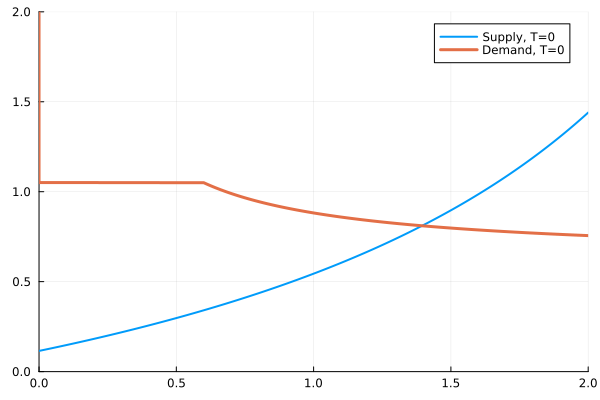
\includegraphics[width=0.7\textwidth]{6c.png}
                \caption{ }
                \label{fig:6c}
        \end{figure}
        \begin{figure}%[H]
            \centering
                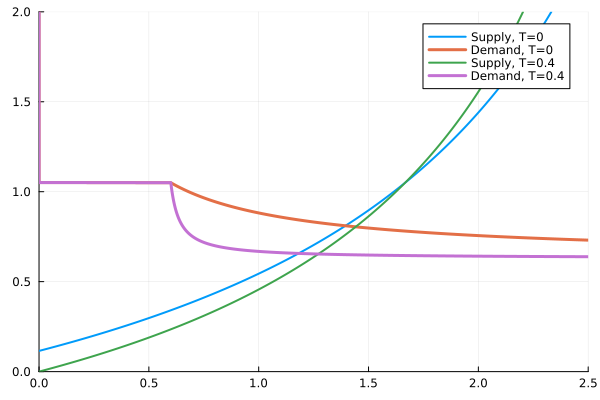
\includegraphics[width=0.7\textwidth]{6c_2.png}
                \caption{ }
                \label{fig:6c2}
        \end{figure}
        
        \item[(d)] {(4 points)} Find the two equilibria by eyeballing the graphs. What are the equilibrium deposit rates before and after the government intervention? By how much did equilibrium deposits change compared to the tax?
        \subsubsection*{Solution.}

        The equilibrium were found at the following and shown in Figure \eqref{fig:6d} and \eqref{fig:6d_d} for equilibrium deposit rates $d$: 

        $T=0$:$ R_d =0.8106, d = 1.3949$
        
        $T=0.4$: $R_d =  0.7609, d = 1.3949$

        Equilibrium deposits change by 0.

        \begin{figure}%[H]
            \centering
                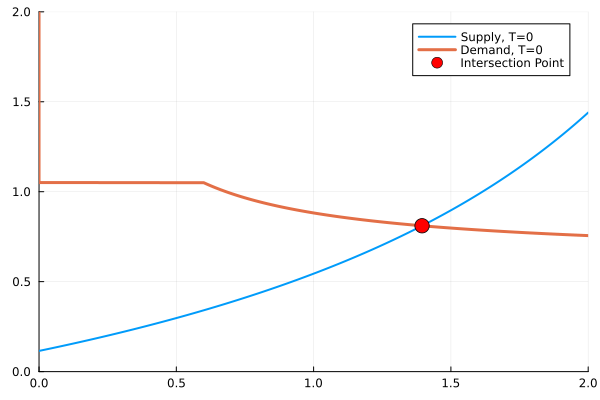
\includegraphics[width=0.7\textwidth]{6d.png}
                \caption{ }
                \label{fig:6d}
        \end{figure}
        \begin{figure}%[H]
            \centering
                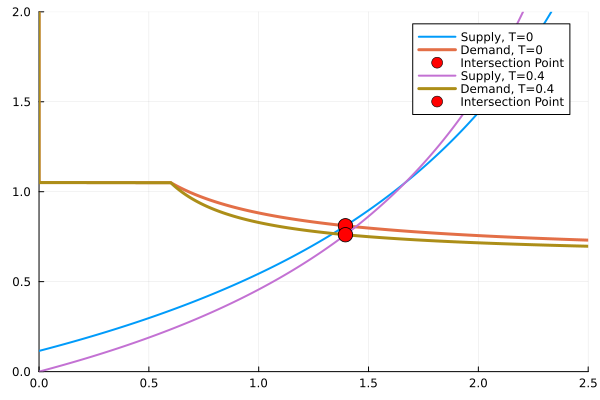
\includegraphics[width=0.7\textwidth]{6d_2.png}
                \caption{ }
                \label{fig:6d_d}
        \end{figure}

        
    \end{enumerate}
\newpage
\item[7.] (25 points) Households comprise workers and bankers. Workers earn $y = 4$ in period 1, bankers make profits $\pi$ in period 2 and both types perfectly insure each other’s consumption. Households have preferences over consumption $c_t$
    \[
    u(c_1, c_2) = \frac{1 - e^{-\alpha c_1}}{\alpha} + \beta \frac{1 - e^{-\alpha c_2}}{\alpha},
    \]
    where $\beta = 0.97$, $\alpha = 0.6$ and $e$ is Euler’s number. Households can earn the deposit return $R_d$ in period 2 on deposits $d$ made in period 1. Bankers’ profits comprise the return $R_s = 1.1$ they earn on both their net worth $N = 0.65$ and deposits $d$, less the deposit return they have to pay for the latter. Bankers have an incentive to default on deposit repayment if their profits are below a share $\lambda = 0.5$ of their assets in period 2. Find the solution to the household’s problem.
    
    \begin{enumerate}
        \item[(a)] {(5 points)} Find the deposit supply and demand functions.
        \subsubsection*{Solution.}

        

        \underline{Banker's problem.} This problem hasn't changed from the base model discussed in lecture, so we have the demand function 
        \[  d= \begin{cases}
                \frac{1-\lambda}{\lambda}N &R^d = R^s
                \\ \frac{(1-\lambda)R^sN}{R^d - (1-\lambda)R^s} & R^d < R^s
            \end{cases}\]
            wherein $\pi = R^s(N+d)-R^dd.$
            
        \underline{Households problem.}
        \begin{align*}
            &\max_{c_1,c_2,d} u(c_1,c_2) 
            && s.t. &\begin{cases}
                c_1 + d = y & t=1 \\ c_2 = R^d d + \pi & t=2 
            \end{cases}
            \\ &\max_{c_1,c_2,d}  \frac{1 - e^{-\alpha c_1}}{\alpha} + \beta \frac{1 - e^{-\alpha c_2}}{\alpha} && s.t & c_2 = R^d y + \pi - R^d c_1
        \end{align*}
        Taking FOC with respect to  $c_1$:    
        \begin{align*}
            e^{-ac_1} + \beta \frac{\partial }{\partial c_1 }\frac{1 - e^{-\alpha (R^d y + \pi - R^d c_1)}}{\alpha}   &= 0
            \\  e^{-ac_1} - \beta R^de^{-\alpha (R^d y + \pi - R^d c_1)}   &= 0
            \\ \alpha\left(R^{d}y+\pi-R^{d}c_{1}\right)-\alpha c_{1}&=\log\left(\beta R^{d}\right)
            \\ c_{1}&=\frac{\alpha\left(R^{d}y+\pi\right)-\log\left(\beta R^{d}\right)}{\alpha(R^{d}+1)} 
            \\ c_{1}&=\frac{\alpha\left(R^{d}y+R^{s}(N+d)-R^{d}d\right)-\log\left(\beta R^{d}\right)}{\alpha(R^{d}+1)} & \text{(plug in $\pi$)}
            \\ d = y - c_1  &= y - \frac{\alpha\left(R^{d}y+R^{s}(N+d)-R^{d}d\right)-\log\left(\beta R^{d}\right)}{\alpha(R^{d}+1)} 
            \\ c_2 = R^d d + \pi &=  R^{s}\left(N+d\right)
        \end{align*}

        Solving for the supply curve $d$:
        \begin{align*}
           % d  &= \frac{R^{d}y\left(1-\alpha\right)-\alpha R^{s}N+y-\log\left(\beta R^{d}\right)}{R^{d}\left(1-\alpha\right)+\alpha R^{s}+1}
           \alpha (R^d+1)d &= \alpha (R^d+1)y - \alpha \Bigl(R^d\,y+R^sN+(R^s-R^d)d\Bigr) + \ln(\beta R^d)
           \\ \alpha (R^d+1)d + \alpha (R^s-R^d)d &= \alpha\Bigl[(R^d+1)+(R^s-R^d)\Bigr]d = \alpha\,(1+R^s)d
           \\\alpha\,(1+R^s)d &= \alpha\,y - \alpha\,R^sN + \ln(\beta R^d)
           \\ d&=\frac{\alpha\,(y-R^sN)+\ln(\beta R^d)}{\alpha\,(1+R^s)}.
        \end{align*}

        So we have the  deposit supply and demand functions: 
        \begin{empheq}[box=\fbox]{align*}
           d  &= \frac{\alpha\,(y-R^sN)+\ln(\beta R^d)}{\alpha\,(1+R^s)}& (supply)
           \\ d&= \begin{cases}
            \frac{1-\lambda}{\lambda}N &R^d = R^s
            \\ \frac{(1-\lambda)R^sN}{R^d - (1-\lambda)R^s} & R^d < R^s
            \end{cases} & (demand)
        \end{empheq}

        \item[(b)] {(5 points)} Plot the deposit supply and demand functions in Julia. Plot $R_d$ on the y-axis for a range from 0 to 2, choose a reasonable scale for deposits on the x-axis. Include your code.
        \subsubsection*{Solution.}

        See Figure \eqref{fig:7b}.

        \begin{figure}%[H]
            \centering
                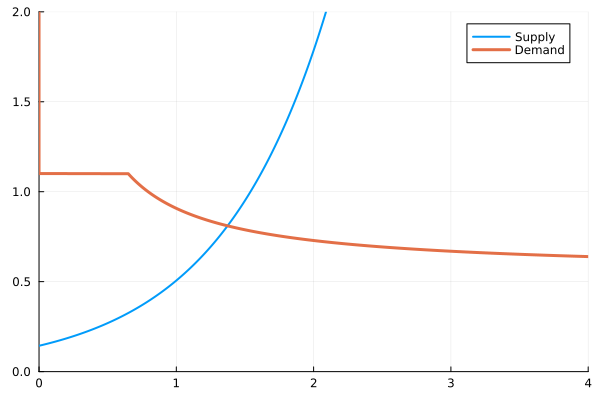
\includegraphics[width=0.7\textwidth]{7b.png}
                \caption{ }
                \label{fig:7b}
        \end{figure}
        
        \item[(c)] {(4 points)} Use a computational solver to find the equilibrium deposit level $d_{eq}$ and the equilibrium deposit rate $R_{d,eq}$. Include your code.
        \subsubsection*{Solution.}

        $  R_d = 0.8103,  d   = 1.3731$. See Figure \eqref{fig:7c} to show that $d_{eq}=1.3731$ and $R_{d,eq}=0.8103.$

        \begin{figure}%[H]
            \centering
                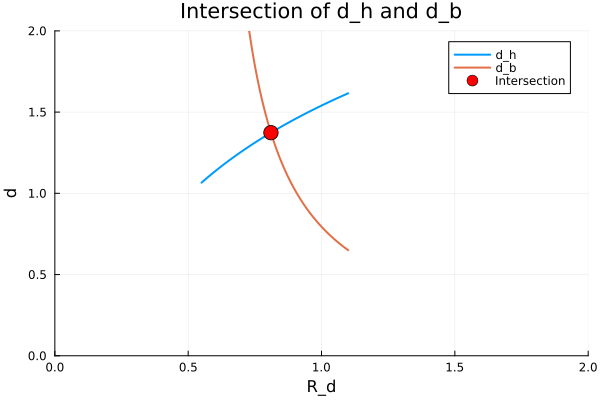
\includegraphics[width=0.7\textwidth]{7c.png}
                \caption{ }
                \label{fig:7c}
        \end{figure}
        
        \item[(d)] {(5 points)} Set up the social planner’s problem in terms of known variables and $d$. Find the first best deposit level $d^*$.
        \subsubsection*{Solution.}

        Since the planner maximizes utility given resources, we have the custom utility for this problem 
        \[ \max_{c_1,c_2,s}   
        u(c_1, c_2) = \max_{c_1,c_2,s}  \frac{1 - e^{-\alpha c_1}}{\alpha} + \beta \frac{1 - e^{-\alpha c_2}}{\alpha} 
        \quad s.t. \quad \begin{cases}
            c_1 + s = y + N & (t=1)
            \\ c_2 = R^ss & (t=2)
        \end{cases} %\iff c_1 = y+N - \frac{c_2}{R^s}
        \]
        Solving the planner's problem: 
        \begin{align*}
           \frac{\partial}{\partial s}: &&  -e^{-\alpha (y + N-s) } + \beta R^s e^{-\alpha R^ss} &= 0
           \\ &&\log\left(\beta R^{s}\right)&=\alpha R^{s}s-\alpha(y+N-s)
        \end{align*}
    
        \begin{empheq}[box=\fbox]{align*}
          s^* &= \frac{\alpha\left(y+N\right)+\log\left(\beta R^{s}\right)}{\alpha\left(R^{s}+1\right)} & \text{(first best loan level to firms)}
        \\ c_1^* &=  y + N- \frac{\alpha\left(y+N\right)+\log\left(\beta R^{s}\right)}{\alpha\left(R^{s}+1\right)} & \text{(first best consumption level)}
        \\c_2^* &= R^s  \frac{\alpha\left(y+N\right)+\log\left(\beta R^{s}\right)}{\alpha\left(R^{s}+1\right)}
        \\ d^* = s-N &= \frac{\alpha\left(y+N\right)+\log\left(\beta R^{s}\right)}{\alpha\left(R^{s}+1\right)}-N & \text{(first best deposit level)} \tag{7. $d^*$}
        \end{empheq}

        \item[(e)] {(2 points)} Calculate the required tax rate $\tau$ to subsidize banks’ interest rates in period 2 in order to achieve the first best.
        \subsubsection*{Solution.}

         \underline{Banker's problem.}
         \begin{align*}
            \max_d \pi =  \max_d R^s(N+d) - R^dd + \tau R^s d^* && s.t. && R^s(N+d) - R^dd + \tau R^s d^*\geq \lambda R^s (N+d)
             \\ &&&&d= \begin{cases}
                \frac{1-\lambda}{\lambda}N+\frac{\tau d^{*}}{\lambda} &R^d = R^s
                \\ \frac{\left(1-\lambda\right)R^{s}N+\tau R^{s}d^{*}}{R^{d}-\left(1-\lambda\right)R^{s}} & R^d < R^s
            \end{cases} 
         \end{align*}
       
            
        \underline{Households problem.}
        \begin{align*}
            &\max_{c_1,c_2,d} u(c_1,c_2) 
            && s.t. &\begin{cases}
                c_1 + d = y & t=1 \\ c_2+ \tau R^s d^* = R^d d + \pi & t=2 
            \end{cases}
            \\ &\max_{c_1,c_2,d}   \frac{1 - e^{-\alpha c_1}}{\alpha} + \beta \frac{1 - e^{-\alpha c_2}}{\alpha}  && s.t & c_2=R^{d}\left(y-c_{1}\right)+\pi-\tau R^{s}d^{*}
        \end{align*}
        Taking FOC with respect to  $c_1$:    
        \begin{align*}
            %e^{-ac_1} + \beta \frac{\partial }{\partial c_1 }\frac{1 - e^{-\alpha (R^d y + \pi - R^d c_1)}}{\alpha}   &= 0
              e^{-ac_1} - \beta R^de^{-\alpha \left(R^{d}\left(y-c_{1}\right)+\pi-\tau R^{s}d^{*}\right)}   &= 0
            \\ \alpha\left(R^{d}\left(y-c_{1}\right)+\pi-\tau R^{s}d^{*}\right)-\alpha c_{1}&=\log\left(\beta R^{d}\right)
            \\ c_{1}&=\frac{\alpha\left(\pi-\tau R^{s}d^{*}\right)+\alpha R^{d}y-\log\left(\beta R^{d}\right)}{\alpha\left(R^{d}+1\right)}
            \\ &=\frac{\alpha\left(R^{s}(N+d)-R^{d}d+\tau R^{s}d^{*}-\tau R^{s}d^{*}\right)+\alpha R^{d}y-\log\left(\beta R^{d}\right)}{\alpha\left(R^{d}+1\right)}% & \text{(plug in $\pi$)}
             \\ &= \frac{\alpha\left(R^{d}y+R^{s}(N+d)-R^{d}d\right)-\log\left(\beta R^{d}\right)}{R^{d}+1} 
           % \\ d = y - c_1  &= y - \frac{\alpha\left(R^{d}y+R^{s}(N+d)-R^{d}d\right)-\log\left(\beta R^{d}\right)}{R^{d}+1} 
            %\\ c_2 = R^d d + \pi &=  R^{s}\left(N+d\right)
        \end{align*}
        Hence, we have the same $c_1,d,c_2$ curves as in the original problem in 7 (a):
        \begin{align*}
            d  &= \frac{R^{d}y\left(1-\alpha\right)-\alpha R^{s}N+y-\log\left(\beta R^{d}\right)}{R^{d}\left(1-\alpha\right)+\alpha R^{s}+1}
            \\ c_2 = R^d d + \pi &=  R^{s}\left(N+d\right)
        \end{align*}

        Now we solve for $\tau$ using the first best deposit level (7. $d^*$) such that  
        \begin{align*}
            R^s(N+d^*) - R^dd^* + \tau R^s d^* &= \lambda R^s (N+d^*)
            \\ \tau &= \frac{\left(\lambda-1\right)N}{d^{*}}+\left(\lambda-1\right)+\frac{R^{d}}{R^{s}}
            \\ &= \frac{\left(\lambda-1\right)N}{\frac{\alpha\left(y+N\right)+\log\left(\beta R^{s}\right)}{\alpha\left(R^{s}+1\right)}-N}+\left(\lambda-1\right)+\frac{R^{d}}{R^{s}}
             \\ &= \frac{\alpha\left(R^{s}+1\right)\left(\lambda-1\right)N}{\alpha\left(y+N\right)+\log\left(\beta R^{s}\right)-N\alpha\left(R^{s}+1\right)}+\left(\lambda-1\right)+\frac{R^{d}}{R^{s}}
        \end{align*}
        
        \item[(f)] {(4 points)} Plot how the tax subsidy alters deposit supply and demand. Use Julia to make this plot and include your code. Where is the new equilibrium?
        \subsubsection*{Solution.}

        The function now plots the first best allocation for demand and supply curves. See Figure \eqref{fig:7f}.

        \begin{figure}%[H]
            \centering
                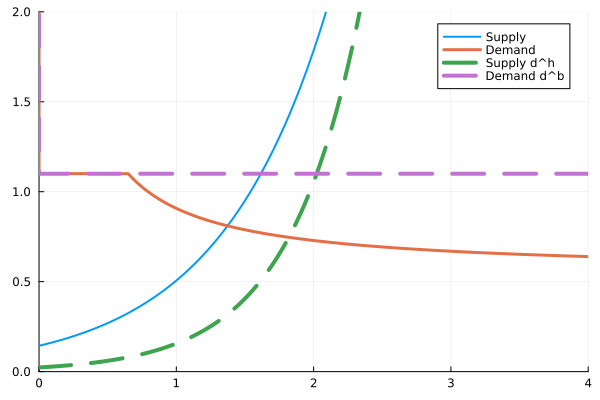
\includegraphics[width=0.7\textwidth]{7f.png}
                \caption{ }
                \label{fig:7f}
        \end{figure}
        
        
    \end{enumerate}

\end{enumerate}
\end{document}
